In order to make the operation more smooth, all the program environment and settings are completed and included in the file package. Just required to follow the steps below to run the program.
\begin{enumerate}

\item Open the package and find the Information System Project.exe file. Double-click the file to enter the program interface as below exactly.
\begin{center}
    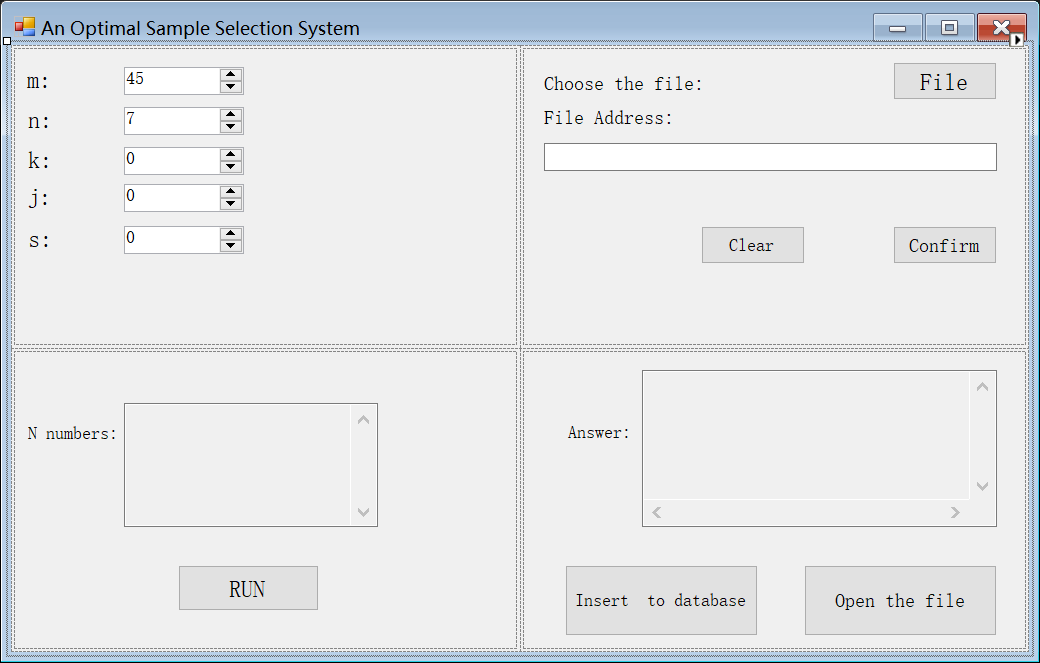
\includegraphics[width=10cm,height=6cm]{images/initial.png}
\end{center}

\item In order to record the relevant output data of the program and facilitate display and modification later. It is required to have a .mdb file to store it, which is called ---.mdb in project package.

\item Choose the data of each parameter and input on the program surface.
\begin{center}
    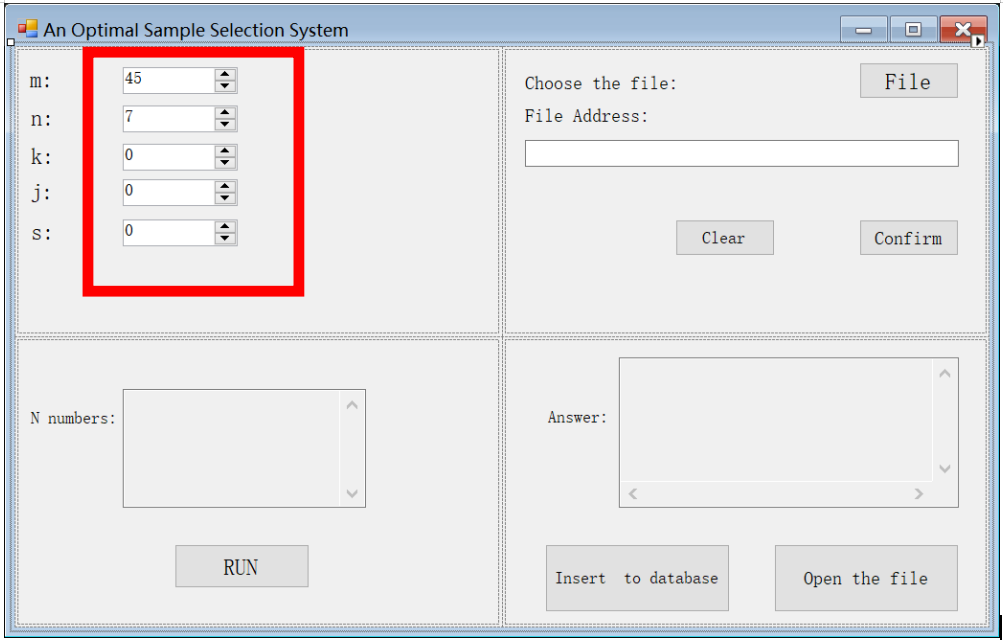
\includegraphics[width=10cm,height=6cm]{images/step1.PNG}
\end{center}

\item Choose the DB file to store and operate the data, click the 'File' and choose the ---.mdb in the previous step and 'Confirm' if all get right.(\textit{'clear' is a function that clear all the data you have input, include the parameter in step 3})
\begin{center}
    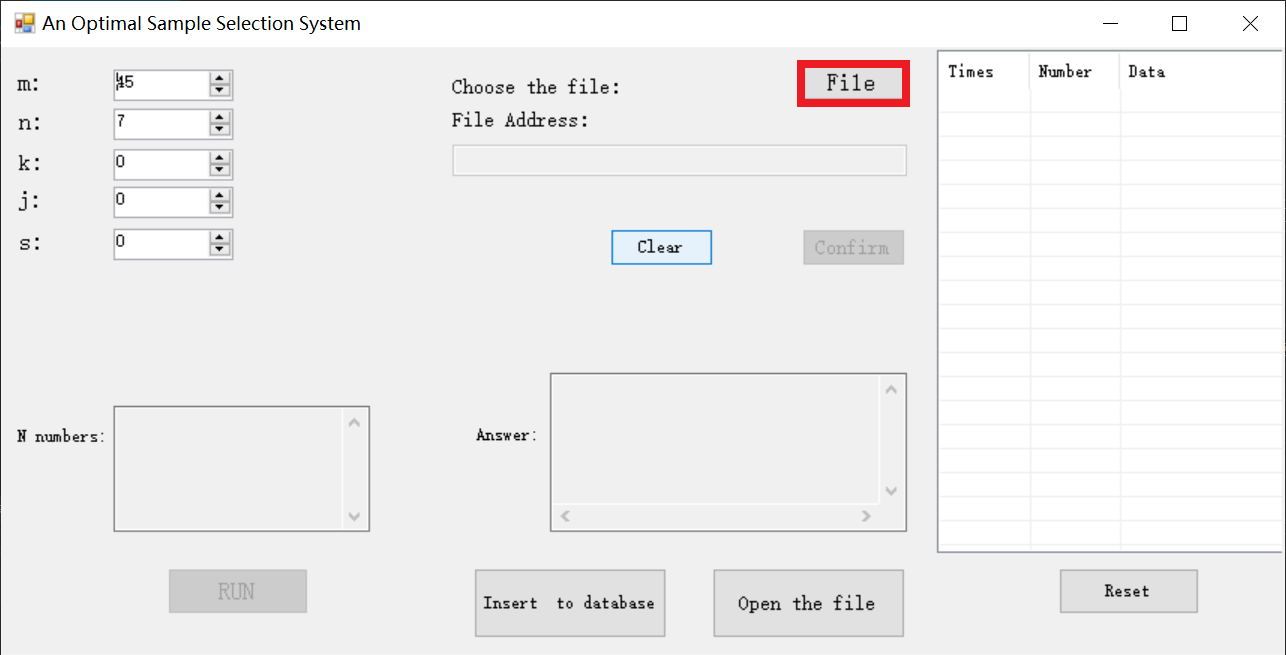
\includegraphics[width=10cm,height=6cm]{images/step2.PNG}
\end{center}
\begin{center}
    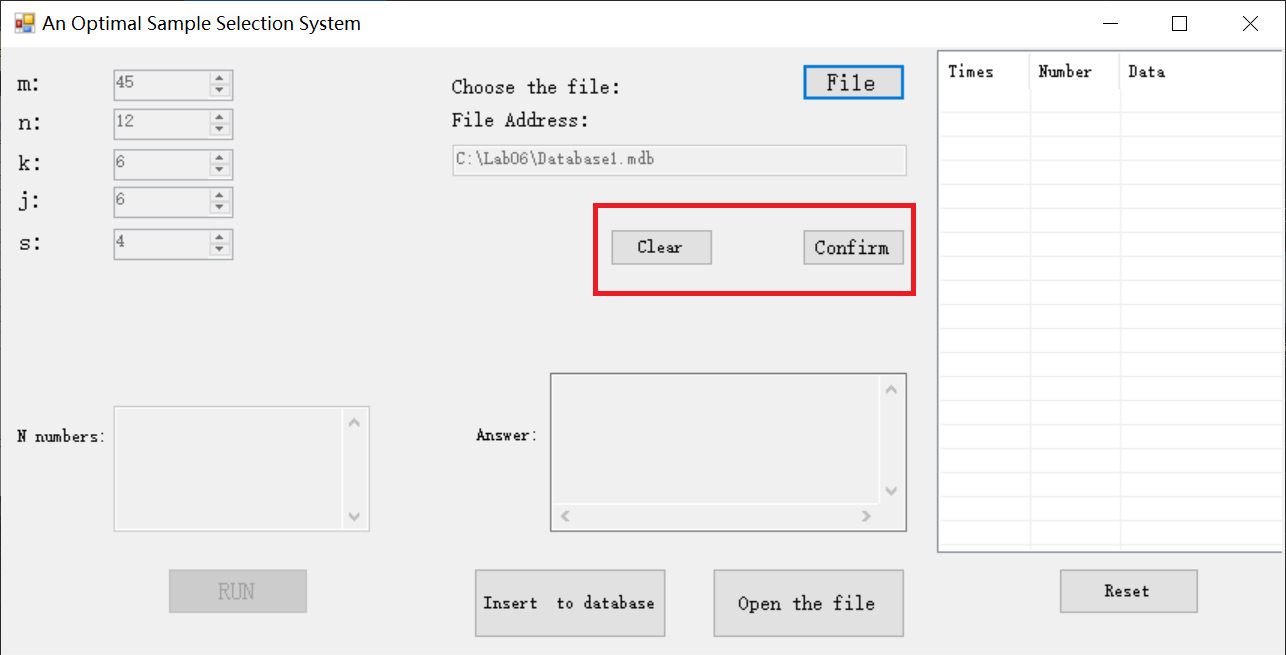
\includegraphics[width=10cm,height=6cm]{images/step3.PNG}
\end{center}

\item Push the 'RUN' button and the N number and final answer of your input will be shown on the surface window, you can check the answer after that.
\begin{center}
    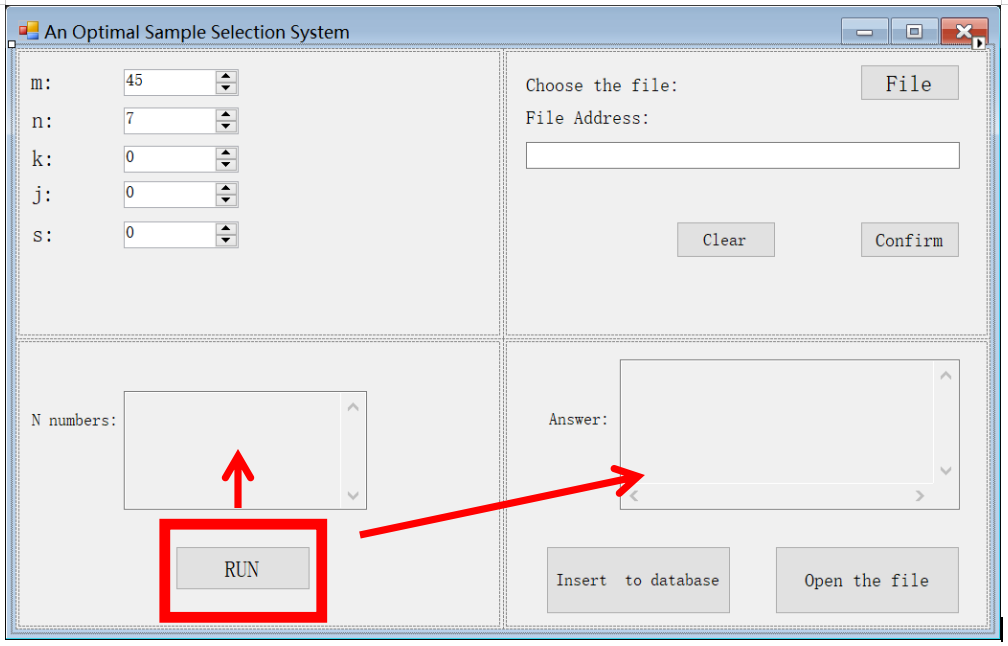
\includegraphics[width=10cm,height=6cm]{images/step4.PNG}
\end{center}

\item After confirm the data is correct, use 'Insert to database' to download the data on the DB file(---.mdb), and 'Open the file' can open it to display the data you have calculate. It is also easy for you to delete or use any other operation on the data though your DB file.
\begin{center}
    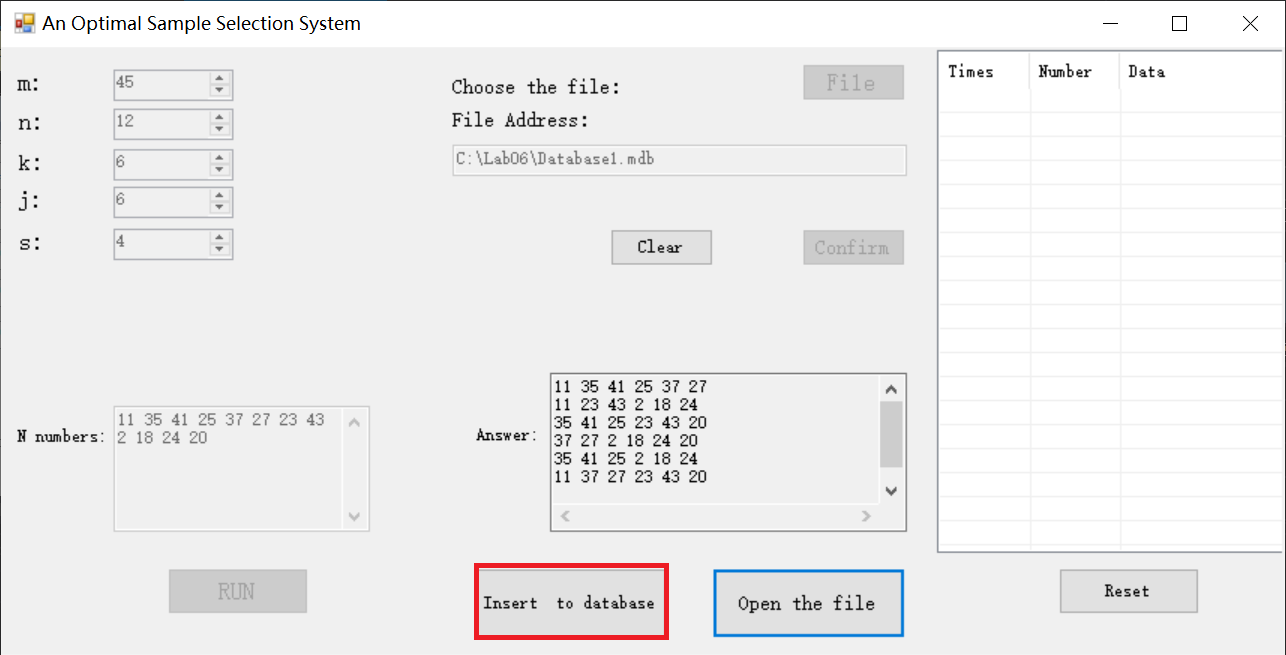
\includegraphics[width=10cm,height=6cm]{images/step5.PNG}
\end{center}
\begin{center}
    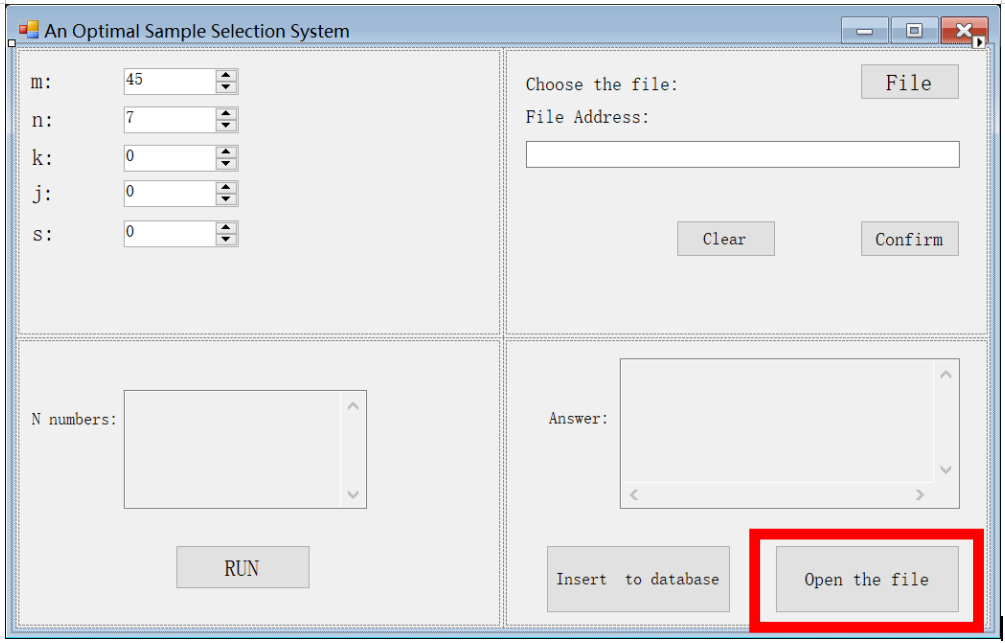
\includegraphics[width=10cm,height=6cm]{images/step6.PNG}
\end{center}

\end{enumerate}